\chapter{Using QTHardMon}

QTHardMon lets you to read in and modify register values of individual boards/cards on your crate. The QTHardMon GUI can list out all registers available for a card along with the current content in these registers. It lets you write custom values to these registers as well (where applicable), thus letting you customize functionality in your cards.

\section{Specifying your crate through the .dmap file}
Before the software can be used, the user has to create a .dmap file. The contents of this file lets the software know about the current set of cards plugged in to the crate. Once a correctly written .dmap file is loaded, the software can list out the cards and their internal registers. An example .dmap file could be as below:

\begin{lstlisting}
# filename: example_crate.dmap
card1    /dev/mtcadummys0 ./mtca_card_registers.map
card2    /dev/llrfdummys4 ./llrf_card_registers.map
\end{lstlisting}


The first line beginning with the \# indicates a comment. 

Line 2 and 3 \todo{fix line numbering in the listing} of the \textit{example\_crates.dmap} file indicates that the user wants to configure a crate that has two cards plugged in- \textit{/dev/mtcadummys0} and \textit{/dev/llrfdummys4} (\textit{/dev/mtcadummys0} and \textit{/dev/llrfdummys4} are device file identifiers \todo{check and correct this terminology if wrong} for these cards). The software displays these cards in the GUI using 'aliases' defined by the user in the .dmap file. In our example the alias names for cards represented by \textit{/dev/mtcadummys0} and \textit{/dev/llrfdummys4} are card1 and card2. Once \textit{example\_crates.dmap} is loaded, the cards will be referred to as card1 and card2 in the GUI.
mtca\_card\_registers.map and llrf\_card\_registers.map are the 'register mapping files' from the firmware \todo{check validity and correct} for \textit{/dev/mtcadummys0} and \textit{/dev/llrfdummys4} respectively. 

Thus, essentially the .dmap file is made up of lines in the following syntax:
\begin{lstlisting}
<card_alias>  <card_device_file_identifier> <path_to_map_files>
\end{lstlisting}

\section{Loading the crate configuration / .dmap file}
Once the cards on your crate have been specified through the .dmap file, the next step is loading this configuration on to the GUI (Fig \ref{load_boards_button} and Fig \ref{load_boards_open_menu_to_load_dmap}). This is done using the "Load Boards" button on the GUI or using the menu option under File > Load Boards:

\begin{figure}[htbp]
\centering
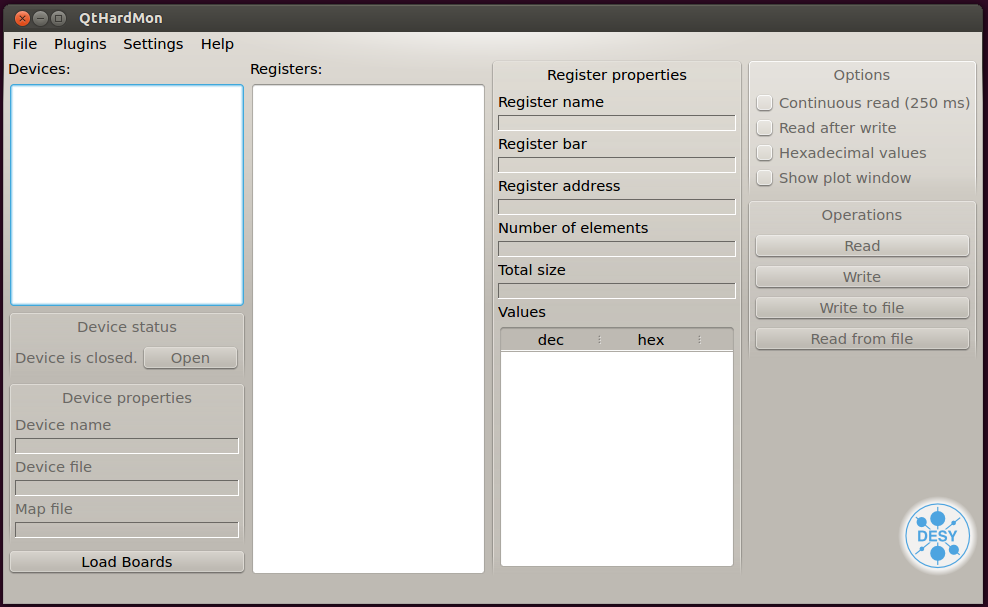
\includegraphics[width=1\textwidth]{images/load_boards_1.png}
 \caption{Loading the .dmap file}
\label{load_boards_button}
\end{figure}

\begin{figure}[htbp]
\centering
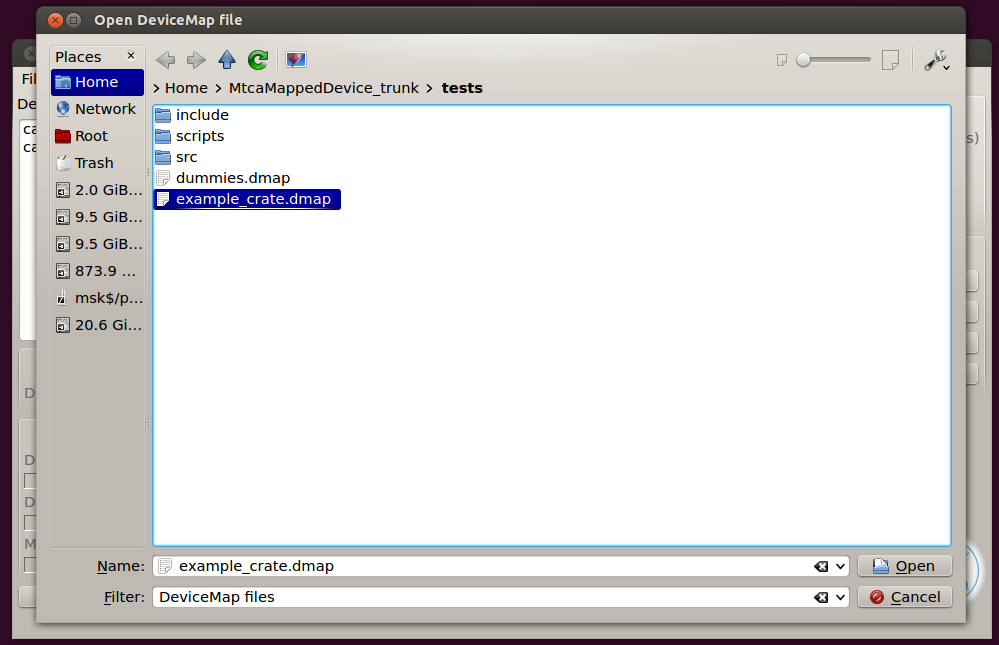
\includegraphics[width=1\textwidth]{images/load_boards_2.png}
 \caption{Loading the .dmap file}
\label{load_boards_open_menu_to_load_dmap}
\end{figure}

\begin{figure}[htbp]
\centering
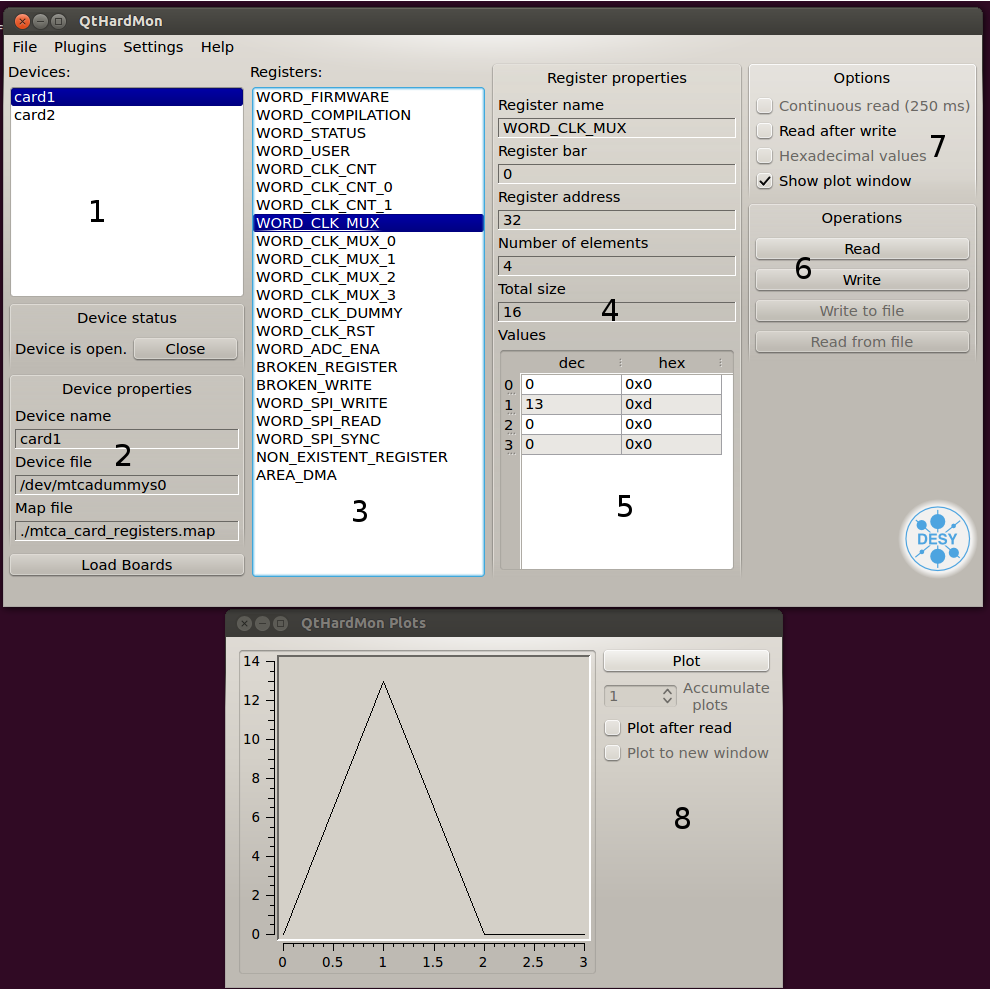
\includegraphics[width=1\textwidth]{images/explain_windows.png}
 \caption{The QtHardMon Interface}
\label{qthardmon_interface}
\end{figure}

\subsection{The QtHardMon Interface}
Information on the induvidual cards become available in the GUI once the .dmap file has been loaded(as seen in Fig \ref{qthardmon_interface}). The GUI has sections that display information on the cards in the crate and these are numbered as in Fig \ref{qthardmon_interface}. The numbered components of the QtHardMon Interface are as below:
\begin{enumerate}
\item \textbf{Devices List:} This section displays the list of cards that were specified in the user defined .dmap file. The user can click on the listed alias names to select induvidual cards and then modify/display properties of that particular card. 
\item \textbf{Device Status and Properties:} Gives an option to open or close a particular card and provides information on the cards device identifier and register mapping file\todo{Check Terminology}.
\item \textbf{Register List:} This part of the GUI displays all registers of the card that are accesible to the user.
\item \textbf{Register Properties:} The properties of the currently selected register is shown here. The properties displayed here include the register name, the PCI express base address range (Register bar), the register address, number of 32 bit words in the register and register size in bytes respecteively.
\item \textbf{Register Values:} The current value present inside the register is displayed here. This field can also be used to set user defined values into the writable registers of the card. The write to a register is done by setting the intended value first in this field and then pressing the write button in the Register Operations section \todo{add a reference here} of the GUI.
\item \textbf{Register Operations:} This part has two working buttons, the first named read and the other one named write. The read button essentially fetches the current value inside the selected register when pressed.

The write button is needed because writing to a register using the GUI, is a two step process. The first step is selecting the register on the card and setting the desired value in the Register Value field and the second part is actually triggering the write to the card by pressing the write button. The value is written only if the write button is pressed, else it gets discarded when the user moves on to select another register/card. 
\item \textbf{GUI options:} If the checkbox titled 'Read after Write' is selected, the GUI actually performs a read from the register and refreshs the display with this value once the write button is clicked. The second checkbox named 'Show plot window' opens a new display window when checked. The function of this  plot window is explained below.
\item \textbf{Plot Window:} The plot window can be used to draw graphs, using the data contained in the registers. The x-axis of the plot is the number of data points/32 bit elements the register contains and the y-axis is the value of those elements. 

The GUI by default generates a plot (for the selected register) only after the plot button is clicked. This default behavior may be modified by setting the 'Plot after read' checkbox in the Plot Window. Selecting this option triggers plotting of the register values, once the register name is clicked or selected using the arrow keys. 

(By defaut the GUI performs an implicit read of the register values from the card when clicking/selecting the register. This is the reason why the checkbox option 'Plot after read' triggers plotting of the register values when register is selected. A thing to note is that the GUI can be set to disable this implicit read when clicking/selecting the register name. The option to do this is in the preferences menu (see section \todo{reference to the prefrence section}). If these implicit read options are disabled in the prefrences, then selecting the 'Plot after read' option will trigger the plot only after the read button is clicked.)
\end{enumerate}

\subsection{Reading and Writing To a Register}
see \todo{Reference to Register Values section}

\subsection{The Prefrences Menu}
The QtHardMon prefrences are under settings>preferences. (Fig \ref{qthardmon_preferences})

\begin{figure}[htbp]
\centering
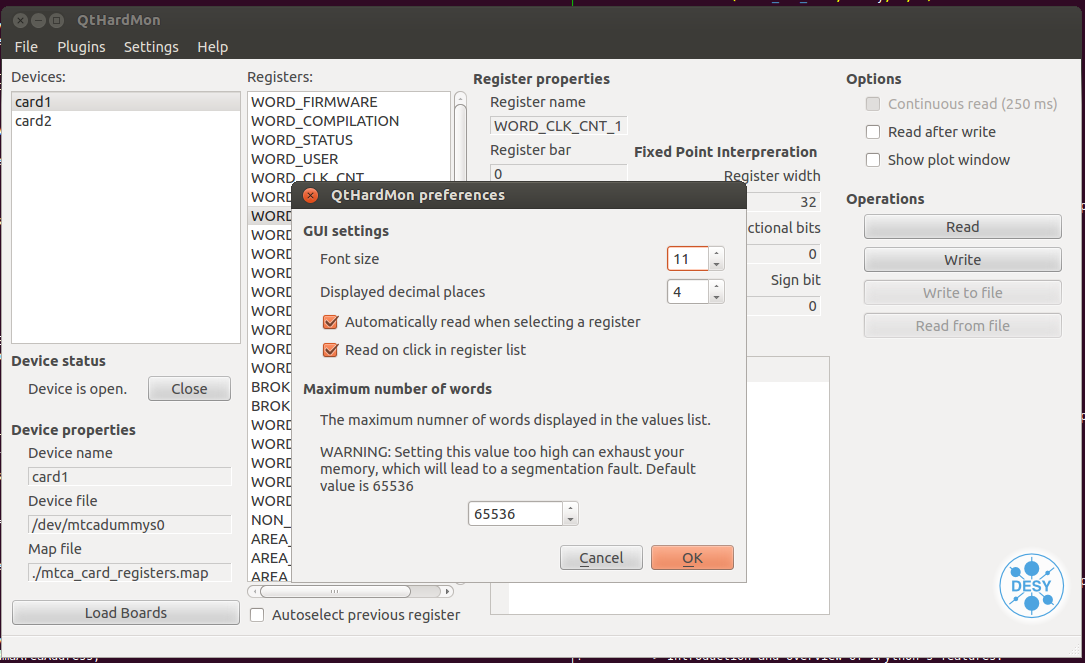
\includegraphics[width=1\textwidth]{images/preferences.png}
 \caption{The QtHardMon Preferences}
\label{qthardmon_preferences}
\end{figure}


% info is displayed in three windows as in fig 2 (labelled as 1, 2, 3)
%
%
%dicates tha
%basically it is the list of boards that the user is planning to put into each slot position of the crate. each is mapped to some .map  file.

%configured through a .dmap file 

%
%Load boards
%This software does this and this for you?
%Create a crate config make your changes and get it back later. So u can have different crate configurations that u can build up. Modify register value on the cards and get  stuff done.
%
%Future revisons of the software would like to keep your changes persistent. Why coz u can load up and u r ready to go. Dont have to reprovision stuff again. 
%
%Creating the .dmap file
%format
%dummyname /dev/<name> mapping
%
%the dummyname can be
%
%what would I want from a crate.....
%decide on what cards to put in. - freely let u rearrange?
%%< auto detect what cards are plugged in the crate>
%< freely rearrange the crds >
%< Type of cards>




